\documentclass[12pt,a4paper]{article}
\usepackage[utf8]{inputenc}
\usepackage{ctex}
\usepackage[margin=2.5cm]{geometry}
\usepackage{amsmath,amssymb,amsfonts}
\usepackage{graphicx}
\usepackage{float}
\usepackage{booktabs}
\usepackage{natbib}
\usepackage{fancyhdr}
\usepackage{titlesec}
\usepackage{xcolor}
\usepackage{hyperref}
\usepackage{tcolorbox}
\usepackage{algorithm}
\usepackage{algpseudocode}
\usepackage{subcaption}
\usepackage{mathtools}

\DeclareMathOperator*{\argmax}{argmax}
\DeclareMathOperator*{\argmin}{argmin}

% 设置页眉页脚
\pagestyle{fancy}
\fancyhf{}
\setlength{\headheight}{15pt}
\fancyhead[L]{\textnormal{UCloud 2025}}
\fancyhead[R]{\textit{Latent variable — a hypothesis about the unknown reality}}
\fancyfoot[C]{\thepage}
\renewcommand{\headrulewidth}{0.5pt}

% 设置标题格式 - 更简洁的样式
\titleformat{\section}
{\Large\bfseries}{\thesection}{1em}{}
\titleformat{\subsection}
{\large\bfseries}{\thesubsection}{1em}{}

% 设置超链接样式
\hypersetup{
    colorlinks=true,
    linkcolor=black,
    citecolor=black,
    urlcolor=blue
}

\begin{document}

\begin{titlepage}
    \centering
    \vspace*{2.5cm}

    % 中文标题
    {\LARGE\bfseries 隐变量 \par}
    \vspace{0.8cm}
    % 英文副标题
    {\large\itshape 一种对未知现实的猜测\par}

    \vspace{2.5cm}    % 作者信息
    \begin{center}
        \begin{tabular}{ll}
            \textbf{姓名:} & 张子路 \\[0.5em]
            \textbf{学号:} & 2023211744 \\[0.5em]
            \textbf{班级:} & 2023219111 \\[0.5em]
            \textbf{专业:} & 人工智能\\[0.5em]
        \end{tabular}
          \vspace{1cm}
    \end{center}

    \vspace{3cm}
    \begin{center}
    \rule{0.6\textwidth}{0.5pt}

    \vspace{0.8cm}
    {\large\textit{What we observe is not nature itself, but nature exposed to our method of questioning}}

    \vspace{0.6cm}
    {\large\textit{我们观察到的不是自然本身,而是我们向自然提问的方式}}

    \vspace{0.5cm}
    \textsc{—— Werner Heisenberg}

    \vspace{0.8cm}
    \rule{0.6\textwidth}{0.5pt}
    \end{center}

    \vfill

    {\normalsize\today\par}
\end{titlepage}


% 添加简洁的分割线
\newcommand{\sectionline}{%
    \noindent\makebox[\linewidth]{\rule{0.8\paperwidth}{0.4pt}}
}

% 摘要页
\newpage
\begin{abstract}
本文聚焦于EM和VAE这两种与隐变量相关的模型或算法,深入讨论了其数学原理与直觉理解,并辅以精心设计的可视化结果,有助于读者加深对两种模型或算法的理解。


\textbf{关键词:} 变分自编码器(VAE),最大期望算法(EM),隐变量,概率生成模型
\end{abstract}

\sectionline

\newpage
\tableofcontents

\newpage
\section{引言}
近年来,隐变量模型及相关推断算法已成为机器学习领域的重要研究方向。经典的EM(Expectation-Maximization)算法作为处理含有隐变量的概率模型的标准工具,自1977年由Dempster等人提出以来\cite{Dempster1977},已广泛应用于聚类、降维及不完全数据处理等领域\cite{Do2008}。而李航\cite{LiHang2020} 和周志华\cite{ZhouZhihua2016} 在其经典教材中也详细阐述了EM算法的理论框架及实践应用。此外,Neal与Hinton\cite{Neal1998} 对EM算法的变体与优化做了深入探讨,进一步拓宽了该方法的应用范畴。

近年来,基于变分推断的隐变量模型逐渐兴起,尤其以变分自编码器(Variational Autoencoder,VAE)为代表的深度生成模型得到了广泛关注。Kingma与Welling\cite{Kingma2014,Kingma2019IntroVAE}首次提出VAE框架,通过融合变分推断和神经网络方法,极大地推进了隐变量模型的研究进程。同时,Rezende等人\cite{Rezende2014}提出了随机反向传播方法,使得VAE的训练更加高效。此外,Burda等人\cite{Burda2016}的权重增强自编码器(Importance Weighted Autoencoder)进一步提升了VAE的性能。

VAE作为生成模型不仅具有强大的数据生成能力,也在数据降维和特征表示学习中表现出色\cite{Hinton2006}。然而,Oring等人\cite{Oring2021}发现传统自编码器在潜空间插值时可能导致严重的图像失真,这也促使研究者关注如何更好地构造和调控VAE的潜空间结构\cite{Doersch2016,Kingma2015,VAEGAN2016}。Blei等人\cite{Blei2017}则从统计学的角度总结了变分推断方法,为机器学习领域提供了严格且全面的理论分析。

此外,经典著作如Murphy的《Machine Learning: A Probabilistic Perspective》\cite{Murphy2012}、Bishop的《Pattern Recognition and Machine Learning》\cite{Bishop2006}以及Goodfellow等人的《Deep Learning》\cite{Goodfellow2016}均详细地描述了隐变量模型的理论基础和实现方法。Jordan等人\cite{Jordan1999}则较早地对图模型的变分方法进行了系统介绍,为后续变分推断的发展奠定了理论基础。

综上所述,隐变量模型与相关推断方法已形成丰富的理论和应用体系。本研究将在EM算法与VAE模型的基础上,进一步探讨隐变量的作用机制,并通过实验验证其有效性与实际表现,以期在理论与实践之间构建更紧密的联系。
% 在引言最后添加横线和GitHub链接
\vfill % 将内容推到页面底部
\noindent\rule{\textwidth}{0.4pt} % 添加横线
\begin{center}
    \textbf{项目代码仓库:} \url{https://github.com/ZZL-2005/mcm-report}
\end{center}
\newpage
\section{EM算法}

\subsection{三硬币问题}
我们以各大教材的经典三硬币问题为例子,作为对EM算法的引入。
考虑下面过程定义的随机试验:
\begin{tcolorbox}[
    colback=gray!5,
    colframe=gray!40,
    boxrule=0.5pt,
    arc=3pt,
    left=8pt,
    right=8pt,
    top=6pt,
    bottom=6pt,
    fontupper=\small
]
\textit{
一共有三枚硬币,A,B,C。单独投掷时,正面朝上的概率分别为$p_A$, $p_B$, $p_C$。
每次实验,我们先投掷硬币A,如果A正面朝上,则下一步投掷硬币B,若反面朝上,则下一步投掷硬币C。
观察第二步投掷的结果,若正面朝上,则记为1,反面朝上则记为0。现在我们已经有若干次独立重复实验结果,$o_1,o_2,...,o_n$。($o_i \in \{0,1\}$)但是我们无法观测到中间过程A的状态。
请给出你对参数$\pi =(p_A$, $p_B$, $p_C)$的估计。
}

\end{tcolorbox}
最大化对数似然,就是要最大化观测事实发生的概率。
最大化对数似然的表达式:
\begin{equation}\label{eq:likelihood}
\begin{split}
\max_{\pi}\log p(o_1,o_2,...,o_n) &= \max_{\pi} \sum_{i=1}^n \log p(o_i) \\
&= \max_{\pi} \sum_{i=1}^n \log \sum_{a \in\mathbb{A}}p(o_i,\mathcal{A}=a)\\
&=\max_{\pi} \sum_{i=1}^n \log \sum_{a \in \mathbb{A}}p(o_i|\mathcal{A}=a)p(\mathcal{A}=a)
\end{split}
\end{equation}
细致的数学符号说明请参照附录表格\ref{tab:symbols},为了论述的连贯性,我们不会在过程中对符号含义进行说明。
公式中的概率分布都是有解析表达的,随机变量$\mathcal{A}\sim \text{Bernoulli}(p_A)$。
\begin{equation}\label{eq:prior}
    p(\mathcal{A}=a)={p_A}^a{(1-p_A)^{1-a}}
\end{equation}
对于给定的$\mathcal{A}$,$o_i$的条件分布,在$a$的各个不同取值的时候,结果都是一个伯努利分布。用与伯努利分布类似的方法可以得到:
\begin{equation}\label{eq:conditional}
    p(o_i|\mathcal{A}=a)=(p_B^{o_i}(1-p_B)^{1-o_i})^a(p_C^{o_i}(1-p_C)^{1-o_i})^{1-a}
\end{equation}
带入公式,我们得到了对数似然的参数化解析表达:
\begin{equation}
    \mathcal{L}(\pi)=\sum_{i=1}^n \log \sum_{a \in \mathbb{A}}(p_B^{o_i}(1-p_B)^{1-o_i})^a(p_C^{o_i}(1-p_C)^{1-o_i})^{1-a}{p_A}^a{(1-p_A)^{1-a}}
\end{equation}
接下来就无法继续求解了,直接求偏导是不可行的,log导致了无比复杂的分母出现,并且每一项的分母还不一样,总之,极大似然估计到这里就算不下去了。
回到公式\ref{eq:likelihood},我们先分析单独的对数似然项:
\begin{equation}
     \log p(o_i)=\log p(o_i,\mathcal{A}=a)-\log p(\mathcal{A}=a|o_i)
\end{equation}
等式两侧同时乘一个关于a的分布$q(a)$:
\begin{equation}
    q(a)\log p(o_i)=q(a)\log p(o_i,\mathcal{A}=a)-q(a)\log p(\mathcal{A}=a|o_i)
\end{equation}
等式两侧同时对$a$求和:
\begin{equation}
\log p(o_i)=\sum_{a \in \mathbb{A}}q(a)\log p(o_i,\mathcal{A}=a)-\sum_{a \in \mathbb{A}}q(a)\log p(\mathcal{A}=a|o_i)
\end{equation}
我们接着做一个技巧,引入一个关于$a$的分布$q$:
\begin{equation}\label{eq:lower_bound}
    \begin{split}
\log p(o_i)&=\sum_{a \in \mathbb{A}}q(a)\log \frac{p(o_i,\mathcal{A}=a)}{q(a)}-\sum_{a \in \mathbb{A}}q(a)\log \frac{p(\mathcal{A}=a|o_i)}{q(a)}\\
&=\sum_{a \in \mathbb{A}}q(a)\log \frac{p(o_i,\mathcal{A}=a)}{q(a)}+KL(q||p(\mathcal{A}|o_i))\\
&\geq \sum_{a \in \mathbb{A}}q(a)\log \frac{p(o_i,\mathcal{A}=a)}{q(a)}
\end{split}
\end{equation}
至此我们得到了单次实验对数似然的一个下界,并且等号当且仅当$q(a)=p(\mathcal{A}=a|o_i)$的时候取得。
考虑一种迭代的情况,我们从当前参数出发,计算隐变量后验,并更新q为后验,然后我们接着在q给定的情况下最大化下界代理函数。
\begin{equation}
\begin{split}
\log p(o_i;\pi^{(t+1)}) &\geq \sum_{a \in \mathbb{A}}q_t(a)\log \frac{p(o_i,\mathcal{A}=a;\pi^{(t+1)})}{q_t(a)} \\
&\geq \sum_{a \in \mathbb{A}}q_t(a)\log \frac{p(o_i,\mathcal{A}=a;\pi^{(t)})}{q_t(a)} \\
&= \log p(o_i;\pi^{(t)})
\end{split}
\end{equation}
其中,$q_t(a)$是当前参数下确定的隐变量后验分布,$\pi^{(t)}$是当前参数。
\begin{gather}
q_t(a) = p(\mathcal{A}=a|o_i;\pi^{(t)})\\
\pi^{(t+1)} = \argmax_{\pi}  \sum_{a \in \mathbb{A}} q_t(a) \log \frac{p(o_i, \mathcal{A}=a;\pi)}{q_t(a)}
\end{gather}
对于所有独立试验的对数似然的总体和式:
\begin{equation}\label{eq:overall_likelihood}
\begin{split}
 \sum_{i=1}^n \log p(o_i|\pi^{(t+1)})&\geq \sum_{i=1}^n \sum_{a \in \mathbb{A}}q_t^i(a)\log \frac{p(o_i,\mathcal{A}=a;\pi^{(t+1)})}{q_t^i(a)} \\
&\geq \sum_{i=1}^n \sum_{a \in \mathbb{A}}q_t^i(a)\log \frac{p(o_i,\mathcal{A}=a;\pi^{(t)})}{q_t^i(a)} \\
&=\sum_{i=1}^n \log p(o_i;\pi^{(t)})
\end{split}
\end{equation}
其中,$q_t^i(a)$是当前参数下第$i$次试验隐变量后验分布,$\pi^{(t)}$是当前参数,此处我们是对每个试验独立更新其隐变量后验。
\begin{gather}
q_t^i(a) = p(\mathcal{A}=a|o_i;\pi^{(t)})\\
\pi^{(t+1)} = \argmax_{\pi}\sum_{i=1}^n  \sum_{a \in \mathbb{A}} q_t^i(a) \log \frac{p(o_i, \mathcal{A}=a;\pi)}{q_t^i(a)}
\end{gather}
下面计算极大化过程式子中的概率项:
\begin{equation}
p(\mathcal{A}=a \mid o_i; \pi^{(t)}) = 
\frac{p(\mathcal{A}=a; \pi^{(t)})}{p(o_i; \pi^{(t)})} = 
\frac{p(o_i \mid \mathcal{A}=a; \pi^{(t)}) \cdot p(\mathcal{A}=a; \pi^{(t)})}
{\sum_{a' \in \mathbb{A}} p(\mathcal{A}=a'; \pi^{(t)}) \cdot p(o_i \mid \mathcal{A}=a'; \pi^{(t)})}
\end{equation}
公式\ref{eq:prior}和\ref{eq:conditional}给出了先验概率和条件概率,带入上式就可以得到目标函数的解析表达:
\begin{equation}
p(\mathcal{A}=a \mid o_i; \pi^{(t)}) = \frac{
    \left(p_A^{(t)}p_B^{(t)})^{o_i}(1 - p_B^{(t)})^{1 - o_i}\right)^a
    \left((1 - p_A^{(t)})p_C^{(t)}{}^{\,o_i}(1 - p_C^{(t)})^{1 - o_i}\right)^{1 - a}
}{
    p_A^{(t)}  p_B^{(t)})^{o_i}(1 - p_B^{(t)})^{1 - o_i}
    + (1 - p_A^{(t)}) p_C^{(t)}{}^{\,o_i}(1 - p_C^{(t)})^{1 - o_i}
}
\end{equation}
\begin{equation}
    \log p(o_i, \mathcal{A}=a;\pi)={p_A}^a{(1-p_A)^{1-a}}(p_B^{o_i}(1-p_B)^{1-o_i})^a(p_C^{o_i}(1-p_C)^{1-o_i})^{1-a}
\end{equation}
考虑到a的取值只有0和1,公式的分段表达更为简洁:
\begin{equation}
p(\mathcal{A}=a|o_i;\pi)=\begin{cases}
\frac{p_B^{o_i}(1-p_B)^{1-o_i}{p_A}}{p_Ap_B^{o_i}(1-p_B)^{1-o_i}+(1-p_A)p_C^{o_i}(1-p_C)^{1-o_i}}, & a=1\\
\frac{(1-p_A)p_C^{o_i}(1-p_C)^{1-o_i}}{p_Ap_B^{o_i}(1-p_B)^{1-o_i}+(1-p_A)p_C^{o_i}(1-p_C)^{1-o_i}}, & a=0
\end{cases}
\end{equation}
\begin{equation}
    \log p(o_i, \mathcal{A}=a;\pi)=\begin{cases}
    \log p_A + o_i\log p_B + (1-o_i)\log(1-p_B), & a=1\\
    \log(1-p_A) + o_i\log p_C + (1-o_i)\log(1-p_C), & a=0
    \end{cases}
\end{equation}
考虑到$q_t^i(a)$实际上对每个试验来讲都是确定的分布,可以简化极大化目标:
\begin{equation}
    \begin{split}
    \pi^{(t+1)} &= \argmax_{\pi}\sum_{i=1}^n  \sum_{a \in \mathbb{A}} q_t^i(a) \log p(o_i, \mathcal{A}=a;\pi)\\
    &=\argmax_{\pi}\sum_{i=1}^n  q_t^i(1) \log p(o_i, \mathcal{A}=1;\pi) + q_t^i(0) \log p(o_i, \mathcal{A}=0;\pi)
    \end{split}
\end{equation}
记目标函数为$E$,对$p_A$求偏导:
\begin{equation}
    \begin{split}
    \frac{\partial E}{\partial p_A} &= \sum_{i=1}^n \left(q_t^i(1) \frac{1}{p_A} - q_t^i(0) \frac{1}{1-p_A}\right)\\
    &=\sum_{i=1}^n \left(\frac{q_t^i(1)}{p_A} - \frac{q_t^i(0)}{1-p_A}\right)
    \end{split}
    \end{equation}
对$p_B$求偏导:
\begin{equation}
    \begin{split}
    \frac{\partial E}{\partial p_B} &= \sum_{i=1}^n \left(q_t^i(1) \frac{o_i}{p_B} - q_t^i(0) \frac{o_i}{1-p_B}\right)\\
    &=\sum_{i=1}^n \left(\frac{q_t^i(1)o_i}{p_B} - \frac{q_t^i(0)o_i}{1-p_B}\right)
    \end{split}
\end{equation}
对$p_C$求偏导:
\begin{equation}
    \begin{split}
    \frac{\partial E}{\partial p_C} &= \sum_{i=1}^n \left(q_t^i(0) \frac{o_i}{p_C} - q_t^i(1) \frac{o_i}{1-p_C}\right)\\
    &=\sum_{i=1}^n \left(\frac{q_t^i(0)o_i}{p_C} - \frac{q_t^i(1)o_i}{1-p_C}\right)
    \end{split}
\end{equation}
解得:
\begin{equation}
\left\{
\begin{aligned}
\frac{\partial E}{\partial p_A} &= \sum_{i=1}^n \left(\frac{q_t^i(1)}{p_A} - \frac{q_t^i(0)}{1 - p_A} \right) = 0 \\
\frac{\partial E}{\partial p_B} &= \sum_{i=1}^n \left( \frac{q_t^i(1)o_i}{p_B} - \frac{q_t^i(1)(1 - o_i)}{1 - p_B} \right) = 0 \\
\frac{\partial E}{\partial p_C} &= \sum_{i=1}^n \left( \frac{q_t^i(0)o_i}{p_C} - \frac{q_t^i(0)(1 - o_i)}{1 - p_C} \right) = 0
\end{aligned}
\right.
\quad \Rightarrow \quad
\left\{
\begin{aligned}
p_A^{(t+1)} &= \frac{1}{n} \sum_{i=1}^n q_t^i(1) \\
p_B^{(t+1)} &= \frac{\sum_{i=1}^n q_t^i(1)o_i}{\sum_{i=1}^n q_t^i(1)} \\
p_C^{(t+1)} &= \frac{\sum_{i=1}^n q_t^i(0)o_i}{\sum_{i=1}^n q_t^i(0)}
\end{aligned}
\right.
\end{equation}
于是,我们可以从一组参数值出发,不断执行先计算后验,然后极大化下界代理函数,如此反复,不断优化观测数据对数似然。
\subsection{实验设置}
\[
\begin{aligned}
&\textbf{真实参数:}\quad
\theta^{\text{true}}=(p_A,p_B,p_C)=(0.1,\;0.9,\;0.3),\\[6pt]
&\textbf{数据生成:}\quad
a_i\sim\mathrm{Bernoulli}(p_A),\quad
o_i\mid a_i\sim
\begin{cases}
\mathrm{Bernoulli}(p_B), & a_i=1,\\
\mathrm{Bernoulli}(p_C), & a_i=0,
\end{cases}
\quad i=1,\dots,1000,\\[6pt]
&\textbf{初始化集合:}\quad
\{\theta_j^{(0)}\}_{j=1}^9
=\bigl\{(0.15,0.85,0.25),\,(0.12,0.92,0.28),\,(0.08,0.88,0.32),\\
&\qquad\qquad\quad\,
(0.90,0.10,0.50),\,(0.80,0.20,0.10),\,(0.20,0.80,0.60),\\
&\qquad\qquad\quad\,
(0.60,0.40,0.90),\,(0.40,0.70,0.20),\,(0.30,0.30,0.80)\bigr\},\\[6pt]
&\textbf{EM 迭代:}\quad t=0,1,\dots,20\text{ 时,先进行 E 步:}\\
&\qquad
q_i^{(t)}
=\frac{p_A^{(t)}\,(p_B^{(t)})^{o_i}(1-p_B^{(t)})^{1-o_i}}
     {p_A^{(t)}\,(p_B^{(t)})^{o_i}(1-p_B^{(t)})^{1-o_i}
      +(1-p_A^{(t)})\,(p_C^{(t)})^{o_i}(1-p_C^{(t)})^{1-o_i}},\\[6pt]
&\qquad\text{然后 M 步更新参数:}\\
&\qquad
p_A^{(t+1)}=\frac{1}{N}\sum_{i=1}^N q_i^{(t)},\quad
p_B^{(t+1)}=\frac{\sum_{i=1}^N q_i^{(t)}\,o_i}{\sum_{i=1}^N q_i^{(t)}},\quad
p_C^{(t+1)}=\frac{\sum_{i=1}^N (1-q_i^{(t)})\,o_i}{\sum_{i=1}^N (1-q_i^{(t)})}.
\end{aligned}
\]
\begin{algorithm}[H]
\caption{EM Algorithm for Three-Coin Model}
\begin{algorithmic}[1]
\Require Observations $\{o_1, o_2, \dots, o_N\} \in \{0,1\}^N$; 
Initialization $\theta^{(0)} = (p_A^{(0)}, p_B^{(0)}, p_C^{(0)})$
\Ensure Estimated parameters $\theta^{(T)}$ after $T$ iterations

\For{$t = 0$ to $T-1$}
    \State \textbf{E-step:} Compute posterior responsibility for each sample:
    \For{$i = 1$ to $N$}
        \State $q_i^{(t)} \gets 
        \dfrac{p_A^{(t)} (p_B^{(t)})^{o_i} (1-p_B^{(t)})^{1-o_i}}
              {p_A^{(t)} (p_B^{(t)})^{o_i} (1-p_B^{(t)})^{1-o_i} + (1-p_A^{(t)}) (p_C^{(t)})^{o_i} (1-p_C^{(t)})^{1-o_i}}$
    \EndFor
    \State \textbf{M-step:} Update parameters:
    \State $p_A^{(t+1)} \gets \dfrac{1}{N} \sum\limits_{i=1}^N q_i^{(t)}$
    \State $p_B^{(t+1)} \gets \dfrac{\sum\limits_{i=1}^N q_i^{(t)} o_i}{\sum\limits_{i=1}^N q_i^{(t)}}$
    \State $p_C^{(t+1)} \gets \dfrac{\sum\limits_{i=1}^N (1 - q_i^{(t)}) o_i}{\sum\limits_{i=1}^N (1 - q_i^{(t)})}$
\EndFor
\State \Return $\theta^{(T)} = (p_A^{(T)}, p_B^{(T)}, p_C^{(T)})$
\end{algorithmic}
\end{algorithm}

\subsection{实验结果}
\begin{figure}[H]
\centering
\begin{subfigure}{0.48\textwidth}
\centering
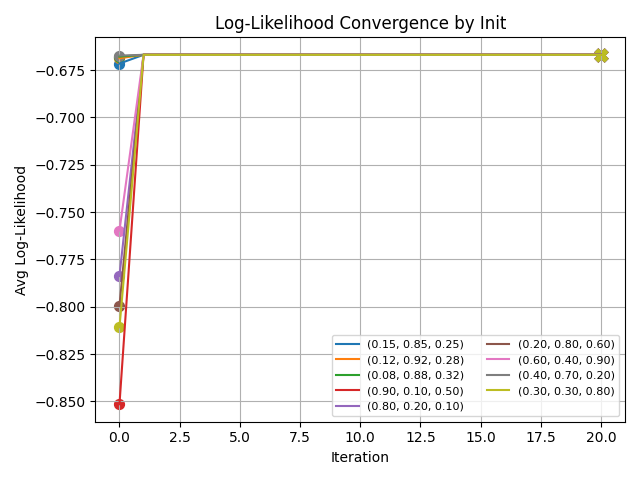
\includegraphics[width=\textwidth]{../images/Figure_2.png}
\caption{对数似然函数收敛过程}
\label{fig:likelihood_convergence}
\end{subfigure}
\hfill
\begin{subfigure}{0.48\textwidth}
\centering
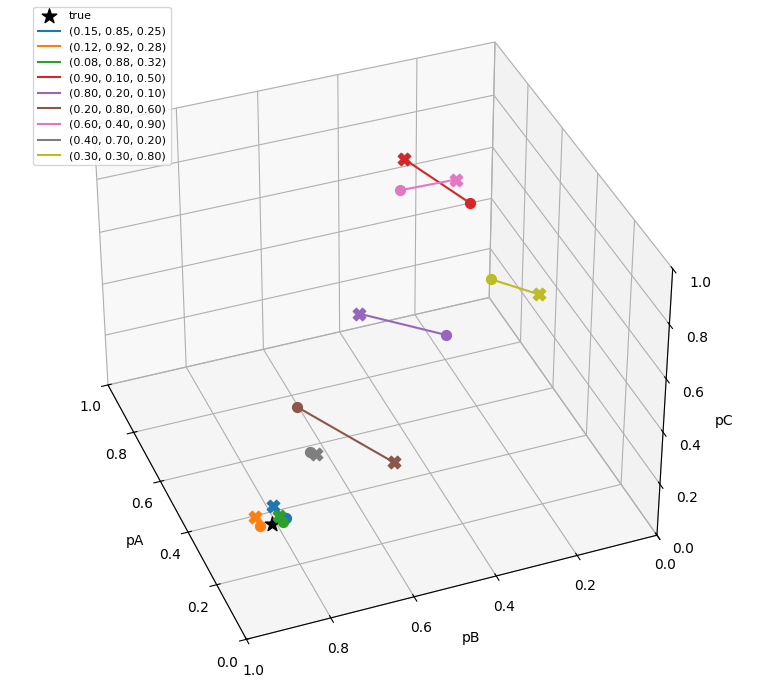
\includegraphics[width=\textwidth]{../images/Figure_1.png}
\caption{参数估计值收敛过程}
\label{fig:parameter_convergence}
\end{subfigure}
\caption{EM算法收敛过程分析}
\label{fig:em_convergence}
\end{figure}
\begin{table}[H]
\centering
\caption{不同初始值下 EM 算法的平均对数似然收敛过程(前5轮)}
\begin{tabular}{lccccc}
\toprule
\textbf{Initial Parameters} & Iter 0 & Iter 1 & Iter 2 & Iter 3 & Iter 4 \\
\midrule
(0.15, 0.85, 0.25) & -0.65894 & -0.65734 & -0.65734 & -0.65734 & -0.65734 \\
(0.12, 0.92, 0.28) & -0.65757 & -0.65734 & -0.65734 & -0.65734 & -0.65734 \\
(0.08, 0.88, 0.32) & -0.65735 & -0.65734 & -0.65734 & -0.65734 & -0.65734 \\
(0.90, 0.10, 0.50) & -0.81703 & -0.65734 & -0.65734 & -0.65734 & -0.65734 \\
(0.80, 0.20, 0.10) & -0.75495 & -0.65734 & -0.65734 & -0.65734 & -0.65734 \\
(0.20, 0.80, 0.60) & -0.81049 & -0.65734 & -0.65734 & -0.65734 & -0.65734 \\
(0.60, 0.40, 0.90) & -0.76749 & -0.65734 & -0.65734 & -0.65734 & -0.65734 \\
(0.40, 0.70, 0.20) & -0.65963 & -0.65734 & -0.65734 & -0.65734 & -0.65734 \\
(0.30, 0.30, 0.80) & -0.82264 & -0.65734 & -0.65734 & -0.65734 & -0.65734 \\
\bottomrule
\end{tabular}
\end{table}
\subsection{实验结果分析}
我们在图中观测到两个有意思的现象,第一,对数似然似乎总是在第一轮就收敛,第二,对数似然在不同初始参数设置下,都收敛到了相同的值。
下面我们从理论上给出对这两个现象的解释。
\subsection{一次收敛现象}

在EM算法的第$t$轮迭代中,E步计算隐变量的后验概率:
\begin{align}
&\text{对于 }o_i=1:\quad
q_t^i(1) = \frac{p_A^{(t)} p_B^{(t)}}{p_A^{(t)} p_B^{(t)} + (1-p_A^{(t)}) p_C^{(t)}} := r_1, \label{eq:r1} \\
&\text{对于 }o_i=0:\quad
q_t^i(1) = \frac{p_A^{(t)} (1-p_B^{(t)})}{p_A^{(t)} (1-p_B^{(t)}) + (1-p_A^{(t)}) (1-p_C^{(t)})} := r_0. \label{eq:r0}
\end{align}

设观测数据中正面出现$n_1$次,反面出现$n_0$次,且$n_1 + n_0 = n$。M步的参数更新公式为:
\begin{equation}
\begin{cases}
p_A^{(t+1)} = \displaystyle\frac{1}{n}\sum_{i=1}^n q_t^i(1) = \frac{n_1 r_1 + n_0 r_0}{n}, \\[8pt]
p_B^{(t+1)} = \displaystyle\frac{\sum_{i=1}^n q_t^i(1) o_i}{\sum_{i=1}^n q_t^i(1)} = \frac{n_1 r_1}{n_1 r_1 + n_0 r_0}, \\[8pt]
p_C^{(t+1)} = \displaystyle\frac{\sum_{i=1}^n (1 - q_t^i(1)) o_i}{\sum_{i=1}^n (1 - q_t^i(1))} = \frac{n_1(1 - r_1)}{n_1(1 - r_1) + n_0(1 - r_0)}.
\end{cases}
\label{eq:m_step}
\end{equation}

现在验证第$t+1$轮E步的后验概率。以$o_i=1$为例:
\begin{align}
q_{t+1}^i(1) &= \frac{p_A^{(t+1)} p_B^{(t+1)}}{p_A^{(t+1)} p_B^{(t+1)} + (1-p_A^{(t+1)}) p_C^{(t+1)}} \notag \\
&= \frac{\displaystyle\frac{n_1 r_1 + n_0 r_0}{n} \cdot \frac{n_1 r_1}{n_1 r_1 + n_0 r_0}}{\displaystyle\frac{n_1 r_1 + n_0 r_0}{n} \cdot \frac{n_1 r_1}{n_1 r_1 + n_0 r_0} + \left(1-\frac{n_1 r_1 + n_0 r_0}{n}\right) \cdot \frac{n_1(1 - r_1)}{n_1(1 - r_1) + n_0(1 - r_0)}} \notag \\
&= \frac{\displaystyle\frac{n_1 r_1}{n}}{\displaystyle\frac{n_1 r_1}{n} + \frac{n_1(1-r_1)}{n}} \notag \\
&= \frac{r_1}{r_1 + (1-r_1)} = r_1 = q_t^i(1).
\label{eq:convergence_proof}
\end{align}

对$o_i=0$的情况同理可得$q_{t+1}^i(1) = q_t^i(1)$。

\textbf{结论}:所有后验概率$q_t^i(a)$在一次EM迭代后保持不变,因此参数更新也停止变化,从而证明了EM算法在此问题上的\textbf{一次收敛}现象。
\subsection{收敛同值现象}

定义样本中观测到正面的比例为:
\begin{equation}
\hat{o} = \frac{1}{n}\sum_{i=1}^n o_i
\end{equation}

对于任意参数三元组$(p_A, p_B, p_C)$,定义边缘概率:
\begin{equation}
\xi = p_A p_B + (1-p_A) p_C
\end{equation}

这表示在整个实验过程中观测到正面结果的总概率。

将完整数据的对数似然函数重新表示:
\begin{align}
\mathcal{L}(p_A, p_B, p_C) &= \sum_{i=1}^n \log p(o_i) \notag \\
&= \sum_{i=1}^n \log[\xi ^{o_i}(1-\xi )^{1-o_i}] \notag \\
&= \sum_{i=1}^n [o_i \log \xi  + (1-o_i) \log(1-\xi )] \notag \\
&= n[\hat{o} \log \xi + (1-\hat{o}) \log(1-\xi )]
\label{eq:likelihood_marginal}
\end{align}

观察:\textbf{对数似然函数仅由边缘概率$\xi $决定},与具体的参数分解$(p_A, p_B, p_C)$无关。

在第$t+1$轮M步中,参数更新满足:
\begin{align}
p_A^{(t+1)} p_B^{(t+1)} &= \frac{\sum_{i=1}^n q_t^i(1) \cdot o_i}{n}, \label{eq:update1} \\
(1-p_A^{(t+1)}) p_C^{(t+1)} &= \frac{\sum_{i=1}^n (1-q_t^i(1)) \cdot o_i}{n} \label{eq:update2}
\end{align}

其中$q_t^i(1) = p(\mathcal{A}=1|o_i; \xi ^{(t)})$是当前参数下硬币A被选中的后验概率。

将公式\ref{eq:update1}和\ref{eq:update2}相加:
\begin{align}
\xi ^{(t+1)} &= p_A^{(t+1)} p_B^{(t+1)} + (1-p_A^{(t+1)}) p_C^{(t+1)} \notag \\
&= \frac{\sum_{i=1}^n q_t^i(1) \cdot o_i}{n} + \frac{\sum_{i=1}^n (1-q_t^i(1)) \cdot o_i}{n} \notag \\
&= \frac{\sum_{i=1}^n [q_t^i(1) + (1-q_t^i(1))] \cdot o_i}{n} \notag \\
&= \frac{\sum_{i=1}^n o_i}{n} = \hat{o}
\label{eq:pi_convergence}
\end{align}

因此,第$t+1$轮的对数似然值为:
\begin{equation}
\mathcal{L}(\xi ^{(t+1)}) = n[\hat{o} \log \hat{o} + (1-\hat{o}) \log(1-\hat{o})]
\label{eq:converged_likelihood}
\end{equation}

\textbf{结论}:无论初始参数$(p_A^{(0)}, p_B^{(0)}, p_C^{(0)})$如何选择,EM算法在第一次迭代后都会将边缘概率$\pi$推向样本比例$\hat{o}$,从而使对数似然收敛到相同的值\eqref{eq:converged_likelihood}。

这解释了实验中观察到的"收敛同值"现象:不同初始化下的EM算法最终都达到相同的对数似然值,因为它们都收敛到了由数据决定的唯一最优边缘概率$\pi = \hat{o}$。
我们可以用我们的实验数据验证一下上面的结论。
\[
\hat{o} \;=\; \frac{1}{n}\sum_{i=1}^n o_i,
\qquad
\mathcal{L}^{\mathrm{exp}}
\;=\;
\hat{o}\,\ln\hat{o} \;+\;(1-\hat{o})\,\ln(1-\hat{o})
\;\approx\;-0.6551.
\]
与实验结果基本吻合,误差是由采样次数有限引起的,因为这次实验和上次实验并不是同一时间执行的,所以1000次采样结果会带来微小差异。
\subsection{事实与观测事实}
由于我们没能观察到隐变量的试验结果,所以我们只好最大化观测事实的似然。
但这毕竟是一种逃避,事实并不是不存在,而只是没有被我们观测到,极大化观测似然是我们的妥协。
妥协也带来了代价,我们并没有得到那个事实上唯一存在的参数值,对于不同的初始参数设置,从图\ref{fig:parameter_convergence}可以看到,我们的收敛结果与事实相差甚远。
这从直觉上就是个极其不合理的算法。我们该如何理解并接受这个妥协呢?
答案在于,\textbf{我们只在意我们看到的事情},我们并不在意事实是什么,我们只在意观测到的事实是什么。
从解释观测事实的角度看,一个错误的收敛结果与一个正确的收敛结果,没有任何本质的不同,它们通过了不同的概率路径,却让我们最终看到了同样的观测事实。

\subsection{下界代理函数}
回顾公式\ref{eq:lower_bound},那里给出了一个重要的不等式:
\begin{equation}
    \log p(o;\pi)\geq \sum_{a \in \mathbb{A}}q(a)\log \frac{p(o,\mathcal{A}=a;\pi)}{q(a)} (\forall q)
\end{equation}
当且仅当$q(a)=p(\mathcal{A}=a|o;\pi)$时,等号成立。
我们可以定义下界代理函数$B(\pi_1,\pi_2)$:
\begin{equation}
    B(\pi_1,\pi_2)=\sum_{a \in \mathbb{A}}p(\mathcal{A}=a|o;\pi_2)\log \frac{p(o,\mathcal{A}=a;\pi_1)}{p(\mathcal{A}=a|o;\pi_2)}
\end{equation}
对数似然总是大于等于其下界代理:
\begin{equation}
    \log p(o;\pi_1)\geq B(\pi_1,\pi_2)
\end{equation}
且当且仅当$\pi_1=\pi_2$时,等号成立。
EM算法迭代的过程可以看成是对下界函数的不断优化,每次先更新赋值$\pi_2$为$\pi_1$,然后对$\pi$极大化$B(\pi,\pi_1)$,得到新的参数估计值。
\subsection{可视化结果}
为了能直观认知这个不断更新下界代理的过程,我们设计了一个双变量的参数估计实验,可视化展示下界代理曲面与对数似然曲面的关系。
\begin{description}
  \item[模型] 观测数据 $\{x_i\}_{i=1}^n$ 服从二元一维高斯混合分布
  \[
    p(x_i\mid\theta)
    =\pi\,\mathcal{N}(x_i;\mu_1,1)
    +(1-\pi)\,\mathcal{N}(x_i;\mu_2,1),
    \quad\theta=(\mu_1,\mu_2)=(-2,2),\;\pi=0.5.
  \]
  \item[数据生成] 隐变量 $z_i\sim\mathrm{Bernoulli}(\pi)$,若 $z_i=1$ 则
  $x_i\sim\mathcal{N}(-2,1)$,否则 $x_i\sim\mathcal{N}(+2,1)$,共采样 $n=100$ 点。
  \item[EM 算法]
    \begin{align*}
      \gamma_i^{(t)}
      &=\frac{\pi\,\mathcal{N}(x_i;\mu_1^{(t)},1)}%
               {\pi\,\mathcal{N}(x_i;\mu_1^{(t)},1)
               +(1-\pi)\,\mathcal{N}(x_i;\mu_2^{(t)},1)},\\
      \mu_1^{(t+1)}
      &=\frac{\sum_{i=1}^n\gamma_i^{(t)}\,x_i}{\sum_{i=1}^n\gamma_i^{(t)}},\quad
      \mu_2^{(t+1)}
      =\frac{\sum_{i=1}^n(1-\gamma_i^{(t)})\,x_i}{\sum_{i=1}^n(1-\gamma_i^{(t)})}.
    \end{align*}
    初始值 $(\mu_1^{(0)},\mu_2^{(0)})=(0,0.5)$,迭代 $T=9$ 轮。
  \item[可视化] 在
  \[
    \min_t\{\mu_k^{(t)}\}-1\;\le\;\mu_k\;\le\;\max_t\{\mu_k^{(t)}\}+1,
    \quad k=1,2
  \]
  区间内构造 $120\times120$ 网格,绘制对数似然面
  $\ell(\mu_1,\mu_2)=\sum_{i=1}^n\log p(x_i\mid\mu_1,\mu_2)$,
  并在其上标注每次迭代点 $(\mu_1^{(t)},\mu_2^{(t)})$ 与收敛路径。
\end{description}
\begin{figure}[H]
  \centering
  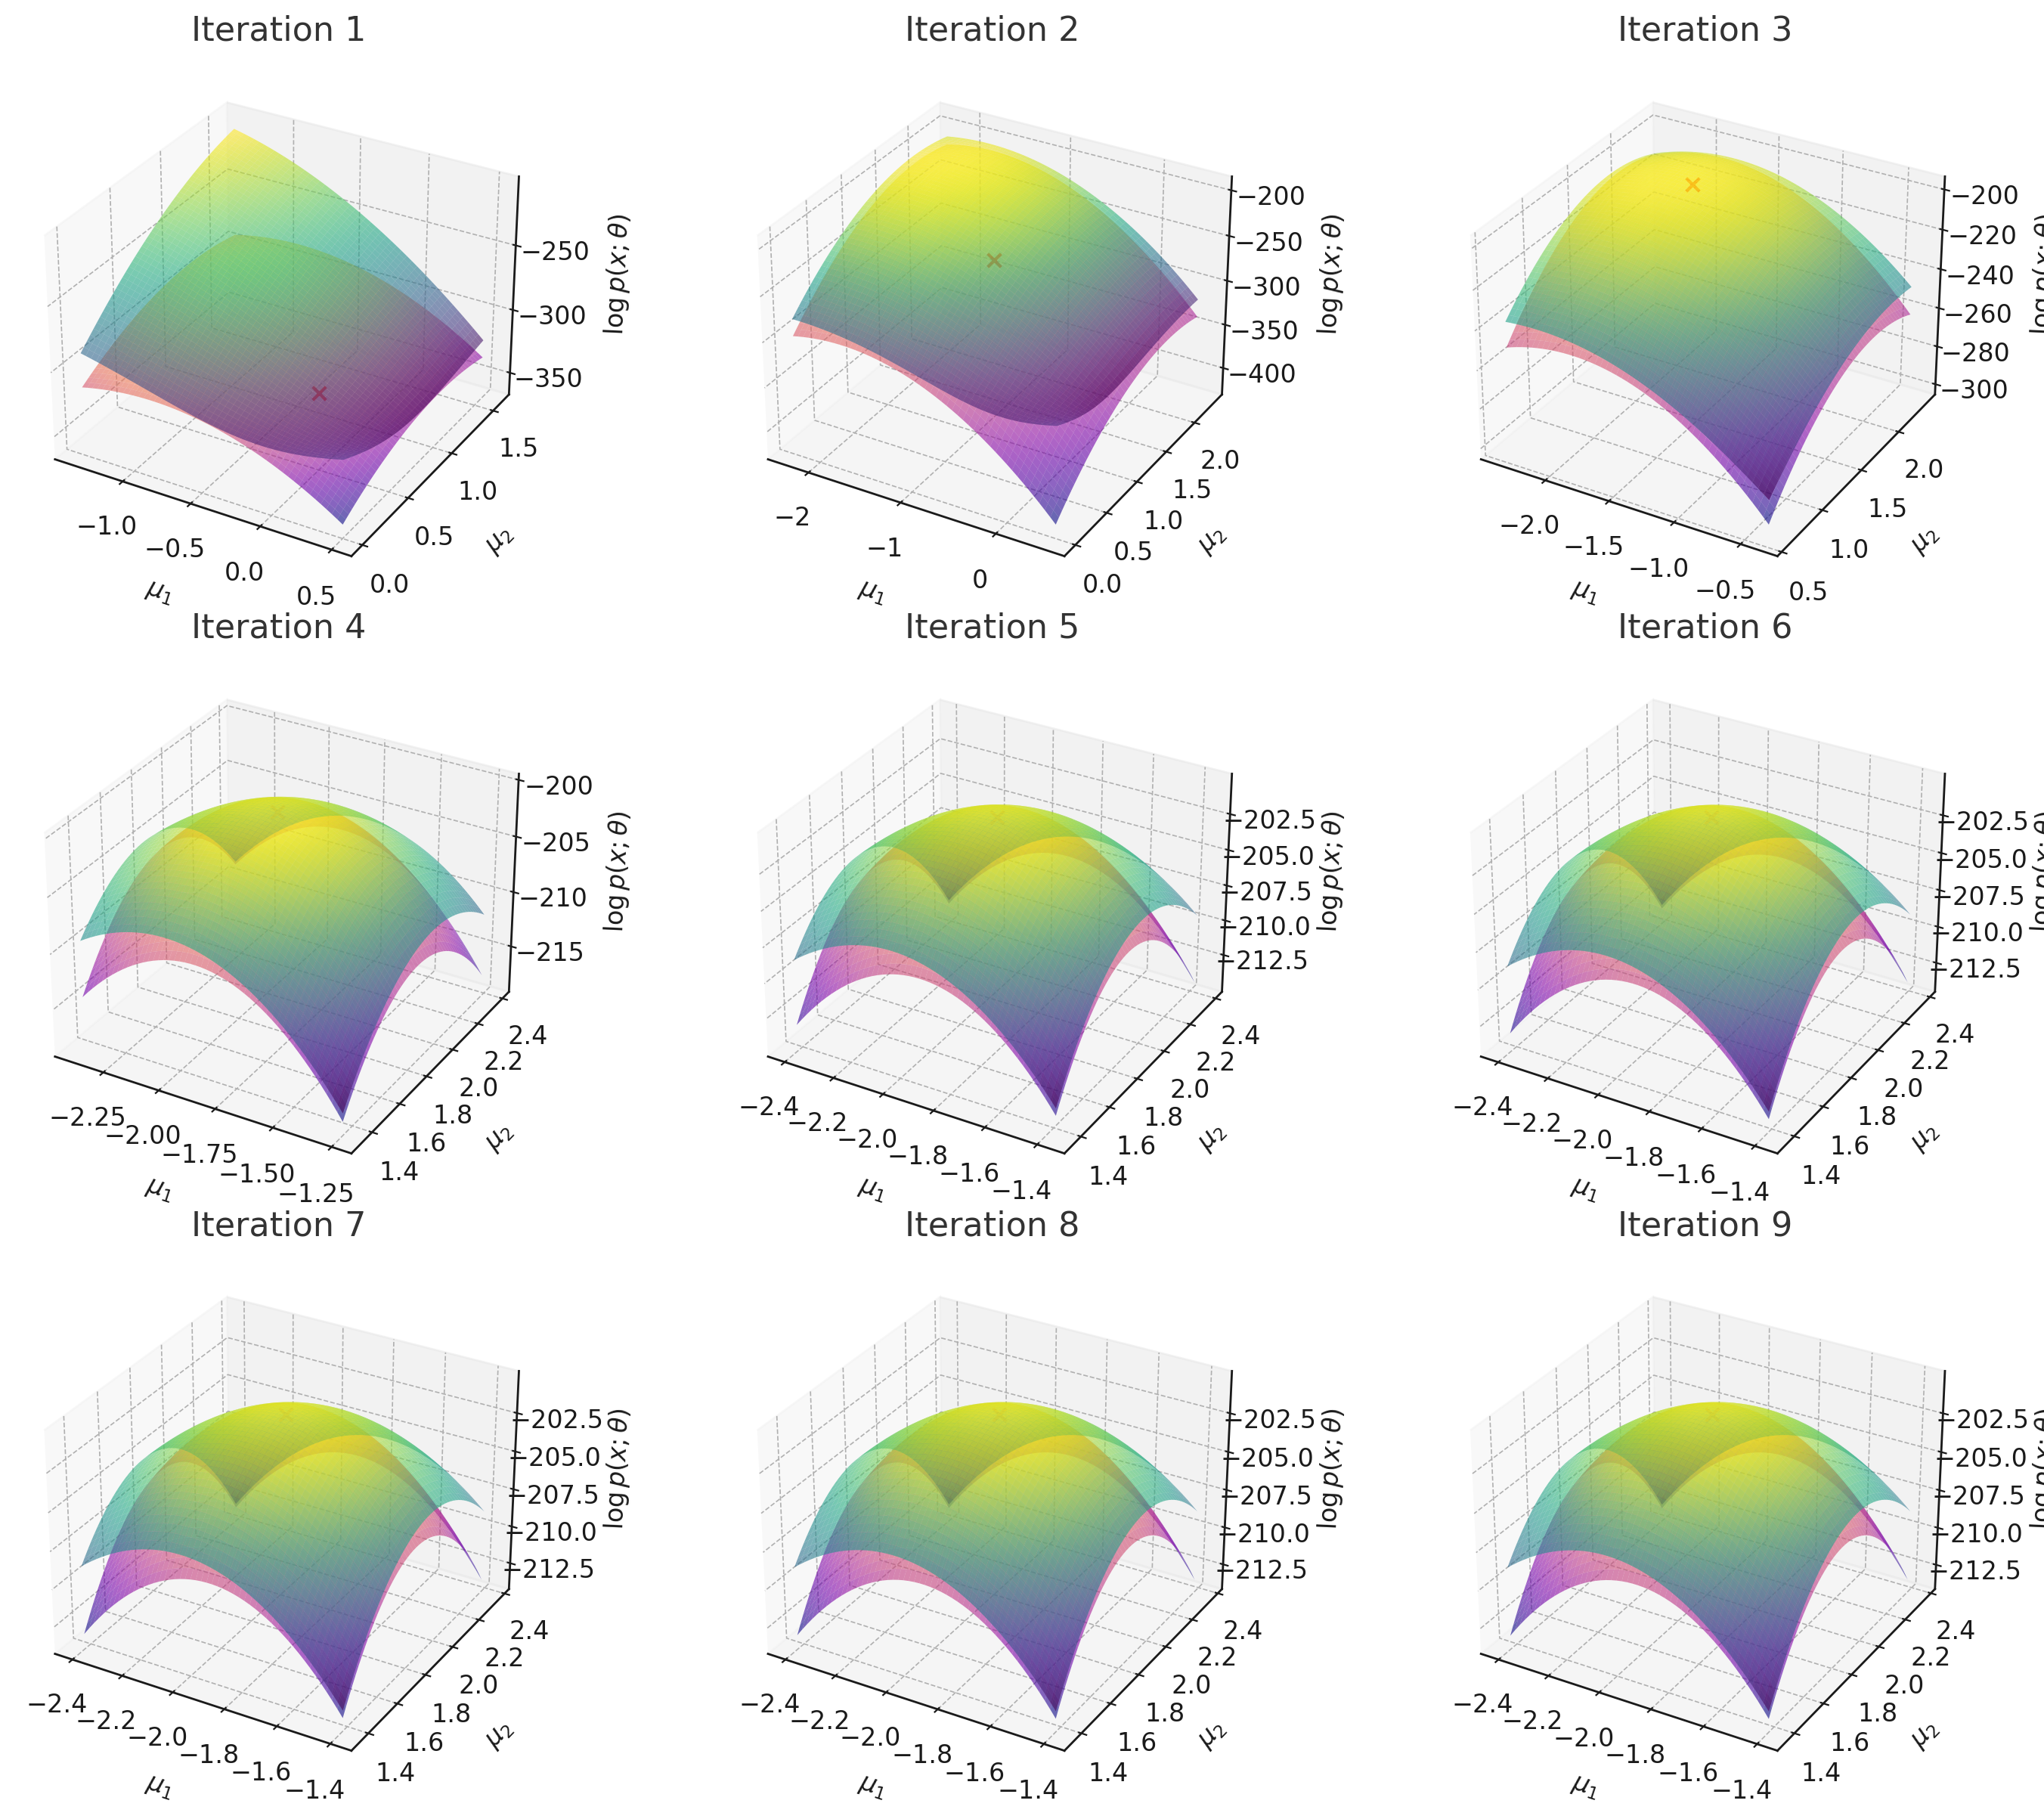
\includegraphics[width=0.75\textwidth]{../images/output1.png}
  \caption{对数似然函数曲面与每一轮的下界代理}
  \label{fig:low}
\end{figure}
\begin{figure}[H]
  \centering
  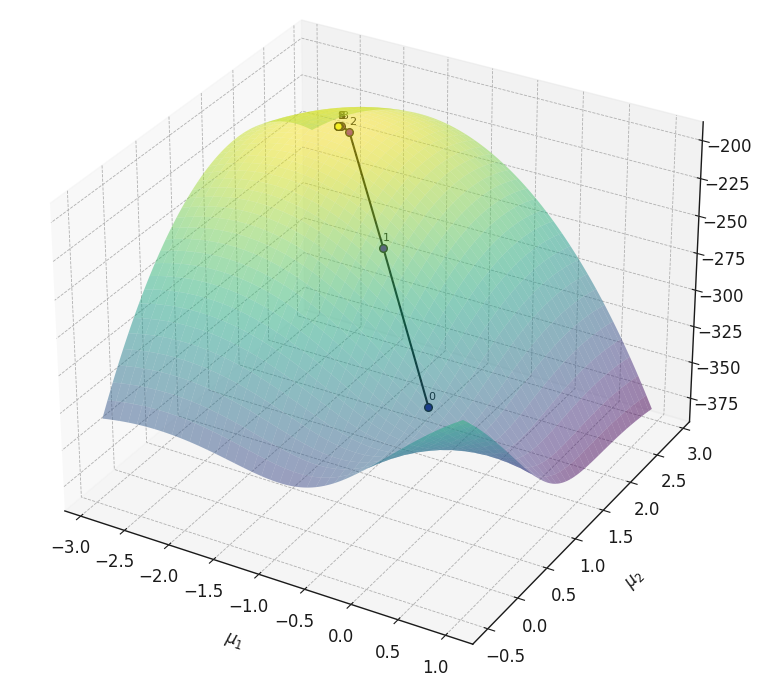
\includegraphics[width=0.75\textwidth]{../images/output2.png}
  \caption{对数似然函数曲面与总体迭代路径}
  \label{fig:likelihood_surface}
\end{figure}
\section{变分自编码器}

\subsection{自编码器}
\begin{figure}[H]
  \centering
  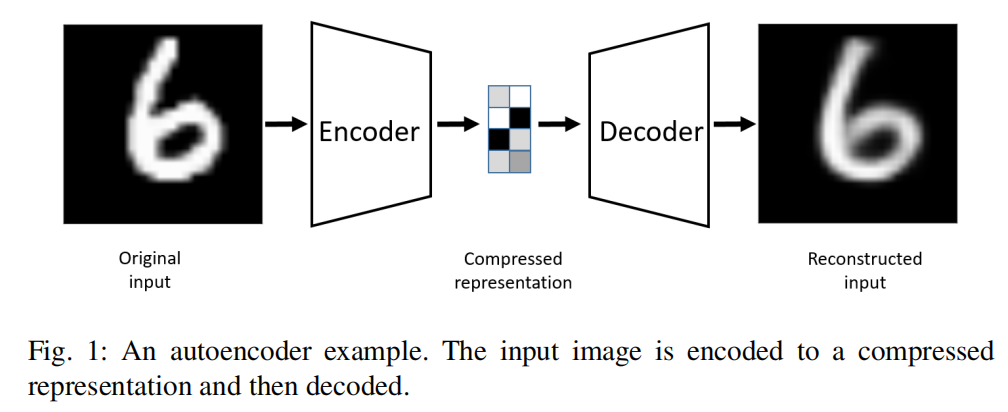
\includegraphics[width=0.75\textwidth]{../images/ae.png}
  \caption{自编码器结构示意图}
  \label{fig:ae}
\end{figure}

自编码器(Autoencoder)是一种典型的无监督神经网络结构,其目标是通过压缩输入数据为低维表示并重构原始输入,从而学习数据的本质特征。

设输入样本为 $x \in \mathbb{R}^n$,编码器函数为 $f(x; \theta_e)$,将其映射为潜在变量 $z \in \mathbb{R}^m$(通常 $m \ll n$);解码器函数为 $g(z; \theta_d)$,用于从潜在空间重构原始输入。则自编码器的整体结构可表示为:
\[
\hat{x} = g(f(x; \theta_e); \theta_d)
\]
其中 $\theta_e$ 和 $\theta_d$ 分别为编码器和解码器的参数。

其训练目标为最小化输入与输出之间的重构误差,常用的损失函数为均方误差(MSE):
\[
\mathcal{L}(\theta_e, \theta_d) = \mathbb{E}_{x \sim p(x)} \left[ \| x - g(f(x; \theta_e); \theta_d) \|^2 \right]
\]

\begin{figure}[H]
  \centering
  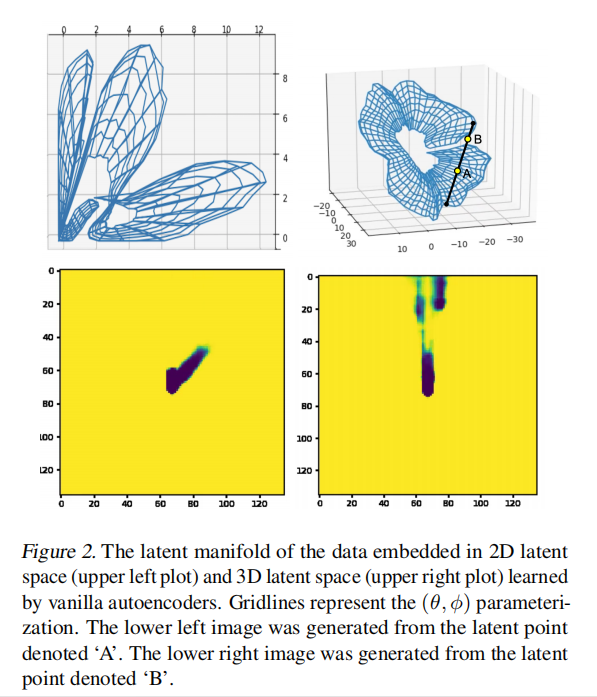
\includegraphics[width=0.75\textwidth]{../images/re1.png}
  \caption{
    引自 Oring 等人(2021)\cite{oring2021interpolation} 的实验结果,展示了原始自编码器(vanilla autoencoder)在潜在空间进行线性插值时可能导致图像失真的问题。
    所用数据为作者构造的一个“竖杆投影”合成图像数据集,通过调节光源的仰角 $\theta$ 与方位角 $\phi$ 控制杆与阴影的位置,图像从固定俯视视角采集。
    图中上排显示了训练样本在 AE 编码后的潜在空间中的嵌入结构,左为二维投影,右为三维视角,均可见其形成一个非凸、弯曲的“花瓣状”网格流形。
    图中点 A 为训练样本的编码位置,解码后(左下)图像自然合理;点 B 为 A 与另一样本之间线性插值得到的 latent 向量,落在流形外部,其解码结果(右下)出现明显畸变。
    作者据此指出:原始自编码器学习到的 latent space 并未与真实数据流形完全对齐,导致插值路径可能穿越“空洞”区域,进而使 decoder 输出失真图像。
  }
  \label{fig:re1}
\end{figure}


\subsection{VAE的插值优势}

\begin{figure}[H]
  \centering
  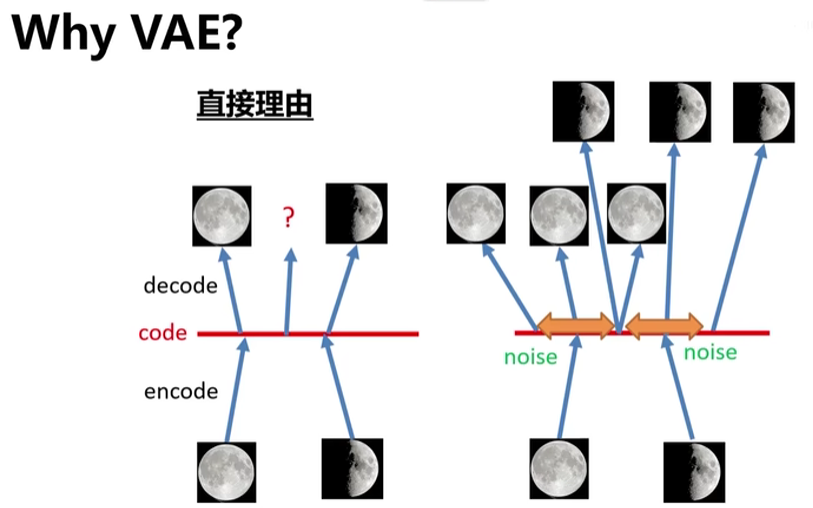
\includegraphics[width=0.75\textwidth]{../images/whyvae.png}
  \caption{VAE的采样操作,能够让解码器隐式学习到潜空间的插值模式}
  \label{fig:chazhi}
\end{figure}
对于一个输入的图像,VAE首先将其编码为一串参数,参数指示了中间层潜空间的后验分布。从分布中采样,我们得到了一个图像的潜空间表示。
由于我们是在分布中采样得到潜变量,所以在潜空间中相近的两个点,他们之间的潜变量的解码结果,会受到这两个点的影响,从而实现了潜空间的插值。
\subsection{模型结构}
\begin{figure}[H]
  \centering
  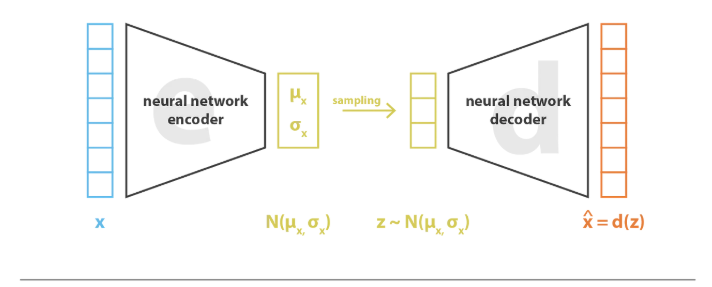
\includegraphics[width=0.75\textwidth]{../images/vae.png}
  \caption{VAE的模型结构示意图}
  \label{fig:vae}
\end{figure}
如图\ref{fig:vae}所示,VAE的模型结构分为编码器和解码器两部分。
相较于AE,VAE从形式上分离了编码器和解码器,两个模块之间通过采样操作连接。
\subsection{数据与潜空间}
为了理解VAE模型,我们首先要从概率生成模型的角度理解潜空间假设。
我们假设现实世界数据如此复杂的结构不是凭空产生的,而是由一些结构更加简单的潜变量通过一系列变换生成的。
从简单结构生成复杂数据是很强的假设,但是正如我们之前所说的,产生观测事实背后的东西也许不可知,但是我们总相信亲眼所见的事实。因此不必纠结于潜空间模型假设,只要它确实能很好地建模事实数据即可。

我们认为隐变量服从一个分布,称之为先验。隐变量通过解码器g生成观测数据,从而确定观测数据的分布。
当给定观测数据,通过编码器f处理,得到隐变量的分布,我们称之为后验。
而模型要学习的,正是如何从数据得到隐变量后验的f,以及如何从隐变量得到观测的g。
这可以看成一个函数拟合问题,VAE使用神经网络作为函数拟合器,拟合f和g。
\subsection{损失函数推导}
对任何的概率生成模型,我们的目标都是一致的,即最大化观测数据的对数似然:
\begin{equation}
    \max_\theta \log p(x;\theta)=\max_\theta  \int_z p(x,z;\theta)dz=\max_\theta  \int_z p(x|z;\theta)p(z;\theta)dz
\end{equation}
这个积分显而易见地难算,比如VAE中,就算z的分布我们设定为简单好算的低维分布,那个条件概率的每次采样,依然要经过神经网络的前向传播,计算量巨大。
但是我们可以和EM算法一样,对对数似然做一个小trick。
\begin{equation}
  \log p(x;\theta)=\log p(x,z;\theta)-\log p(z|x;\theta)
\end{equation}
引入关于z的分布q,并同时对z积分:
\begin{equation}
  \log p(x;\theta)=\int_z q(z)\log p(x,z;\theta)-\int_z q(z)\log p(z|x;\theta)
\end{equation}
接着在分母中引入$q(z)$:
\begin{equation}
  \log p(x;\theta)=\int_z q(z)\log \frac{p(x,z;\theta)}{q(z)}-\int_z q(z)\log \frac{p(z|x;\theta)}{q(z)}
\end{equation}
后面那项加上符号是KL散度,于是得到了对数似然的下界:
\begin{equation}\label{43}
    \log p(x;\theta)\geq \int_z q(z)\log \frac{p(x,z;\theta)}{q(z)}
\end{equation}
\newpage
由式(\ref{43})得到的变分下界可以进一步展开。首先对联合概率进行分解:

\begin{equation}
p(x, z; \theta) = p_\theta(x|z) \cdot p(z) \label{44}
\end{equation}

将其代入变分下界表达式(\ref{43}):

\begin{equation}
\log p(x; \theta) \geq \int q(z) \log \frac{p_\theta(x|z) \cdot p(z)}{q(z)} \, dz \label{45}
\end{equation}

接下来对分子展开对数:

\begin{equation}
\log p(x; \theta) \geq \int q(z) \log p_\theta(x|z) \, dz + \int q(z) \log \frac{p(z)}{q(z)} \, dz \label{46}
\end{equation}

第一个积分项表示在 $q(z)$ 下对 $\log p_\theta(x|z)$ 的期望,第二项即为 $q(z)$ 相对于 $p(z)$ 的 KL 散度。因此,变分下界可以写成:

\begin{equation}
\log p(x; \theta) \geq \mathbb{E}_{q(z)}[\log p_\theta(x|z)] - \mathrm{KL}(q(z) \| p(z)) \label{47}
\end{equation}

这就是变分推断中的证据下界(Evidence Lower Bound, ELBO)。在实际的变分自编码器(VAE)模型中,$q(z)$ 被参数化为 $q_\phi(z|x)$,表示给定样本 $x$ 的编码器输出分布,同时 $p_\theta(x|z)$ 表示解码器的生成模型。于是最终的优化目标为最大化:

\begin{equation}
\mathcal{L}_{\text{ELBO}}(\theta, \phi; x) = \mathbb{E}_{q_\phi(z|x)}[\log p_\theta(x|z)] - \mathrm{KL}(q_\phi(z|x) \| p(z)) \label{48}
\end{equation}

\section{结语}
引入分布q得到变分下界以及用神经网络拟合分布的tricks固然巧妙,但我认为隐变量的假设才是这一切方法的核心。
抛掷硬币的结果背后有着那个硬币A作为控制一切的隐变量,当结果转换为了宏大自然所呈现的一切数据的时候,数据的背后是否也是由某个“硬币A”控制着一切呢?
% 参考文献
\nocite{*}  % 输出所有 BibTeX 条目
\bibliographystyle{plain}  % 或者使用 alpha、ieeetr、unsrt 等风格
\bibliography{ref}




\newpage
\appendix

\section{附录}

\subsection{数学符号说明}
\begin{table}[h]
\centering
\caption{数学符号说明}
\label{tab:symbols}  % 添加这一行
\begin{tabular}{cl}
\hline
\textbf{符号} & \textbf{含义} \\
\hline
\multicolumn{2}{c}{\textbf{基本变量}} \\
\hline
$\mathcal{A}$ & 描述硬币A投掷结果的随机变量\\
$\mathbb{A}$ & 随机变量$\mathcal{A}$的取值集合,本例中为$\{0,1\}$  \\
$o_i$ & 第$i$次观测结果,$o_i \in \{0,1\}$ \\
$n$ & 观测次数 \\
$\hat{o}$ & 样本中正面结果的比例,$\hat{o} = \frac{1}{n}\sum_{i=1}^n o_i$ \\
\hline
\multicolumn{2}{c}{\textbf{参数相关}} \\
\hline
$\pi = (p_A, p_B, p_C)$ & 三个硬币投出正面的概率参数向量 \\
$\pi^{(t)}$ & EM算法第$t$次迭代的参数估计 \\
$\xi$ & 边缘概率,$\xi = p_A p_B + (1-p_A) p_C$ \\
$r_1, r_0$ & 观测到正面/反面时硬币A被选中的后验概率 \\
\hline
\multicolumn{2}{c}{\textbf{函数与分布}} \\
\hline
$L(\pi)$ & 对数似然函数 \\
$q_t^i(a)$ & 第$t$次迭代时观测$o_i$下隐变量$\mathcal{A}=a$的后验概率 \\
$Q(\pi|\pi^{(t)})$ & EM算法中的Q函数(期望完整数据对数似然) \\
$p(o_i, \mathcal{A}=a; \pi)$ & 观测值和隐变量的联合概率 \\
$\mathcal{N}(\mu, \sigma^2)$ & 均值为$\mu$、方差为$\sigma^2$的正态分布 \\
\hline
\multicolumn{2}{c}{\textbf{算法相关}} \\
\hline
$\argmax$ & 使目标函数达到最大值的参数 \\
$\mathcal{L}(q,\theta)$ & 证据下界(ELBO) \\
$\theta$ & 一般参数记号 \\
$T$ & EM算法的迭代次数 \\
\hline
\end{tabular}
\end{table}


\subsection{附加实验}
本附加实验旨在从参数空间的角度直观展示 EM 算法对不同初始值的收敛行为。具体步骤如下:

\begin{enumerate}
  \item 在 $[0.05,0.95]^3$ 范围内均匀采样若干组初始参数 $(p_A,p_B,p_C)$;
  \item 对每组初始值仅执行两步 EM 迭代,记录迭代结束后的收敛点 $\theta_{\rm final}=(p_A,p_B,p_C)$;
  \item 利用径向基函数(RBF)插值,在 $(p_A,p_B)$ 网格上对所有收敛点拟合出平滑曲面 $p_C=f(p_A,p_B)$,从而得到左图所示的“收敛结果曲面”;
  \item 计算每个收敛点在观测数据下的平均对数似然值,并在真参数对应的对数似然水准上应用 marching\_cubes 算法提取三维等值面,得到右图所示的“对数似然等值面”。
\end{enumerate}
\begin{figure}[H]
  \centering
  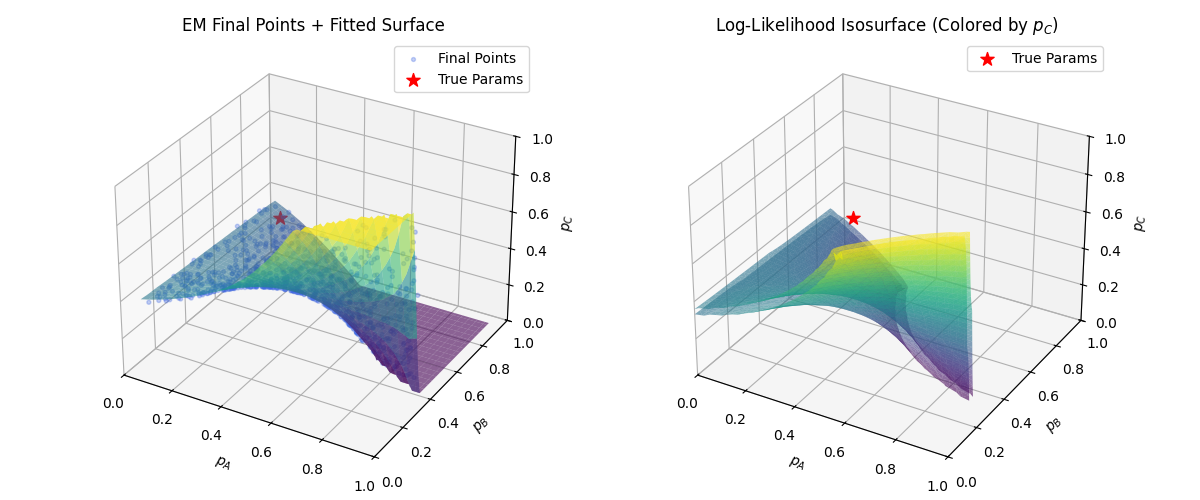
\includegraphics[width=0.75\textwidth]{../images/sur.png}
  \caption{左图为不同初始点导致的不同收敛结果组成的收敛结果曲面,右图为收敛结果对应的似然值导出的对数似然等值面}
  \label{fig:sur}
\end{figure}

\subsection{思维导图}
\begin{figure}[H]
  \centering
  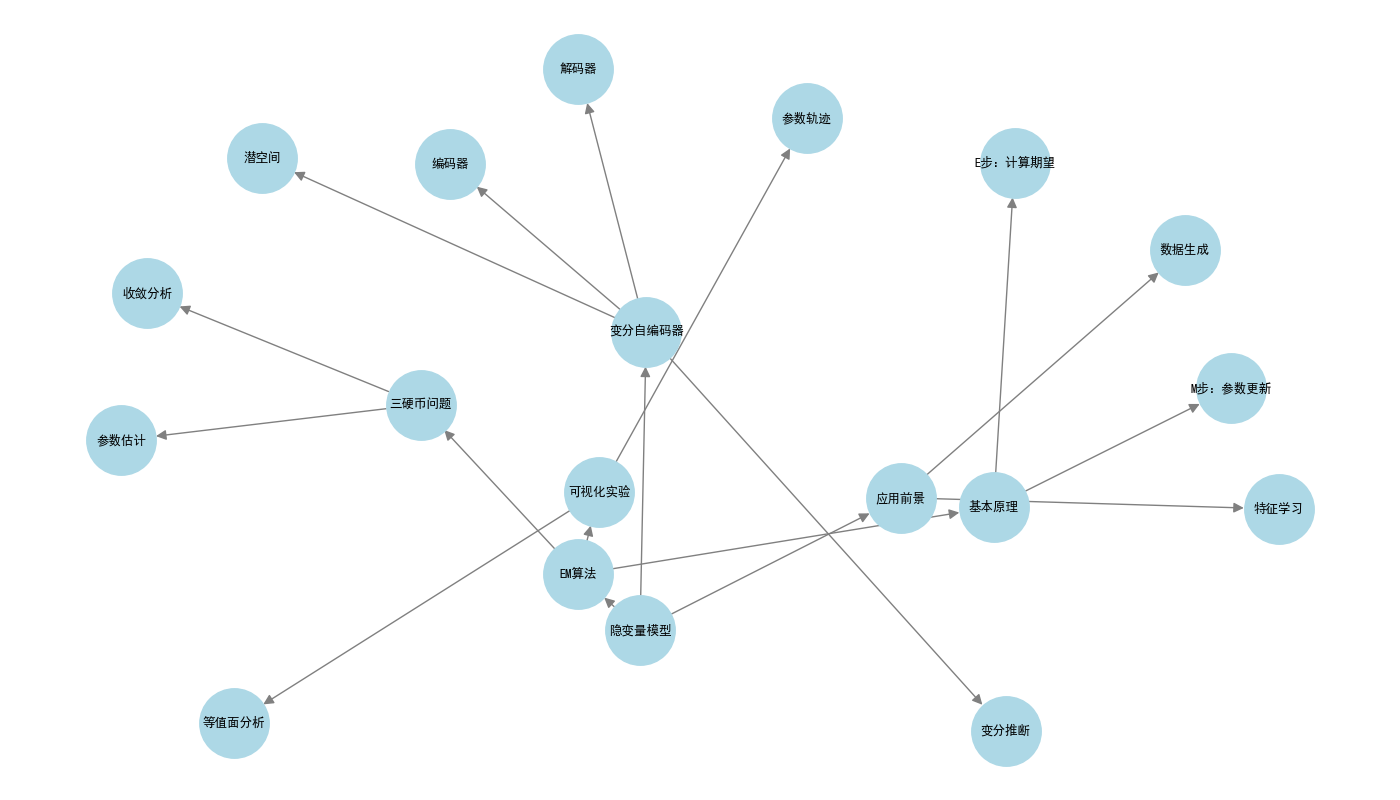
\includegraphics[width=0.75\textwidth]{../images/mind.png}
  \caption{思维导图}
  \label{fig:mind}
\end{figure}

\end{document}